\subsection*{Датчик - треугольное распределение}
\addcontentsline{toc}{subsection}{Датчик - треугольное распределение}

\textbf{Задание:}\\
Для треугольного распределения получить функцию распределения. Используя метод обратной функции, получить последовательность случайных чисел с треугольным распределением. Оценить математическое ожидание и дисперсию, построить гистограмму.\\

\textbf{Решение:}\\
Пусть имеются следующие параметры: $a$ (\textit{min}), $b$ (\textit{max}), $c$ (\textit{мода}).\\
Плотность треугольного распределения:
\begin{ceqn}
	\begin{align*}
		f(x) =
		\begin{cases}
			\dfrac{2(x-a)}{(b-a)(c-a)} \quad , x \in [a,c]\\
			\dfrac{2(b-x)}{(b-c)(b-a)} \quad , x \in [c,b]\\
			0 \hspace{3.25cm} , x \centernot\in [a,b]\\
		\end{cases}
	\end{align*}
\end{ceqn}

Функция распределения треугольного закона:
\begin{ceqn}
	\begin{align*}
		F(x) =
		\begin{cases}
			0 \hspace{4.1cm} , x < a\\
			\dfrac{(x-a)^2}{(b-a)(c-a)} \hspace{1.3cm} , x \in [a,c]\\
			1 - \dfrac{(x-b)^2}{(b-a)(b-c)} \quad , x \in [c,b]\\
			1 \hspace{4.1cm} , x > b\\
		\end{cases}
	\end{align*}
\end{ceqn}

Получается, что обратная функция $F^{-1}(x)$ будет выглядеть следующим образом:
\begin{ceqn}
	\begin{align*}
		F^{-1}(y) = x =
		\begin{cases}
			a + \sqrt{(b-a)(c-a)y} \hspace{2.2cm} , 0 < y < \dfrac{c-a}{b-a}\\
			b - \sqrt{(b-a)(b-c)(1-y)} \hspace{1cm} , \dfrac{c-a}{b-a} \leq y < 1\\
		\end{cases}
	\end{align*}
\end{ceqn}

Если подставить вместо $y$ случайные равномерно распределённые значения, то можно получить требуемые числа.

Таким образом, была реализована функция на языке программирования Python. (Рисунок \ref{fig:triangle_inverse_function_method_code})
\begin{figure}[h]
	\centering 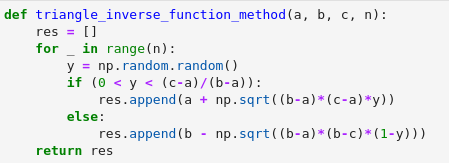
\includegraphics[scale=0.7]{triangle_inverse_function_method_code}
	\caption{Реализация метода обратной функции для треугольного закона}
	\label{fig:triangle_inverse_function_method_code}
\end{figure}

При $a = 0$, $b = 1$, $c = 0.5$ и $n = 10$ получается следующий результат. (Рисунок \ref{fig:triangle_inverse_function_method_result})
\begin{figure}[h]
	\centering 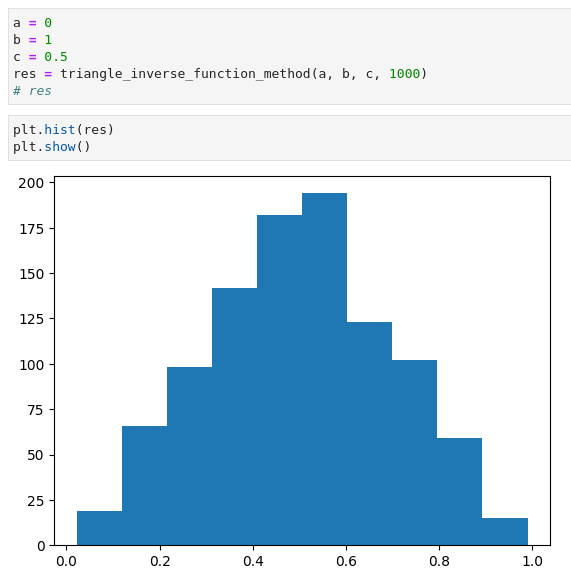
\includegraphics[scale=0.5]{triangle_inverse_function_method_result}
	\caption{Результаты генерации случайных чисел методом обратной функции для треугольного закона}
	\label{fig:triangle_inverse_function_method_result}
\end{figure}

Математическое ожидание треугольного распределения:
\begin{ceqn}
	\begin{align*}
		E = \dfrac{a + b + c}{3}
	\end{align*}
\end{ceqn}
\newpage
Если рассчитывать математическое ожидание как среднее значение в выборке, то получается следующий результат. (Рисунок \ref{fig:triangle_inverse_function_method_math})
\begin{figure}[h]
	\centering 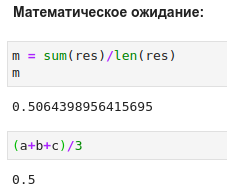
\includegraphics[scale=0.7]{triangle_inverse_function_method_math}
	\caption{Теоретическое и расчётное значения математического ожидания ($a = 0$, $b = 1$, $c = 0.5$)}
	\label{fig:triangle_inverse_function_method_math}
\end{figure}

Можно заметить, что при $n = 1000$ значения получились достаточно близкими.\\
Дисперсия треугольного распределения:
\begin{ceqn}
	\begin{align*}
		D = \dfrac{a^2 + b^2 +c^2 - a \cdot b - a \cdot c - b \cdot c}{18}
	\end{align*}
\end{ceqn}
Далее можно рассчитать дисперсию как среднее квадратное отклонение от среднего значения выборки. (Рисунок \ref{fig:triangle_inverse_function_method_var})
\begin{figure}[h]
	\centering 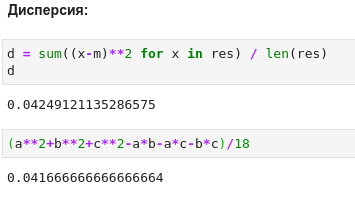
\includegraphics[scale=0.7]{triangle_inverse_function_method_var}
	\caption{Теоретическое и расчётное значения дисперсии ($a = 0$, $b = 1$, $c = 0.5$)}
	\label{fig:triangle_inverse_function_method_var}
\end{figure}

Можно заметить, что при $n = 1000$ значения получились достаточно близкими.

\newpage

Также стоит проверить гипотезу о том, что получившиеся значения распределены по треугольному закону. Для этого воспользуемся критерием Колмогорова-Смирнова. (Рисунок \ref{fig:triangle_inverse_function_method_test})
\begin{figure}[h]
	\centering 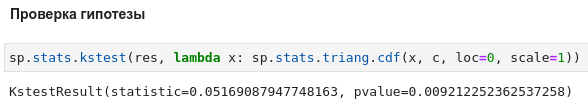
\includegraphics[scale=0.6]{triangle_inverse_function_method_test}
	\caption{Результаты теста Колмогорова-Смирнова}
	\label{fig:triangle_inverse_function_method_test}
\end{figure}

Значение \textit{p-value} > 0.05, значит мы принимаем гипотезу о том, что данная выборка имеет треугольное распределение.